\documentclass[a4paper, table, 11pt]{article}
\usepackage[utf8]{inputenc} % Allows the use of some special characters
\usepackage{amsmath, amsthm, amssymb, amsfonts} % Nicer mathematical typesetting
\usepackage[portuguese]{babel} % Portuguese language settings
\usepackage{setspace}
\usepackage{graphicx} % Allows the use of \begin{figure} and \includegraphics
\usepackage{float} % Useful for specifying the location of a figure ([H] for ex.)
\usepackage{caption} % Adds additional customization for (figure) captions
\usepackage{subcaption} % Needed to create sub-figures
\usepackage{tabularx} % Adds additional customization for tables
\usepackage{tabu} % Adds additional customization for tables
\usepackage{booktabs} % For generally nicer looking tables
\usepackage[nottoc,numbib]{tocbibind} % Automatically adds bibliography to ToC
\usepackage[left=3cm, right=2cm, top=2cm, bottom=2cm]{geometry}
\usepackage{microtype} % Slightly loosens margin restrictions for nicer spacing  
\usepackage{titlesec} % Used to create custom section and subsection titles
\usepackage{titletoc} % Used to create a custom ToC
\usepackage{appendix} % Any chapter after \appendix is given a letter as index
\usepackage{fancyhdr} % Adds customization for headers and footers
\usepackage[shortlabels]{enumitem} % Adds additional customization for itemize. 
\usepackage{hyperref} % Allows links and makes references and the ToC clickable
\usepackage[noabbrev, capitalise]{cleveref} % Easier referencing using \cref{<label>} instead of \ref
\usepackage{xcolor} % Predefines additional colors and allows user defined colors
\usepackage{tikz} % Useful for drawing images, used for creating the frontpage
\usepackage{changepage} % Allows the use of \begin{adjustwidth} and \end{adjustwidth}
\usepackage{listings} % Allows the use of \begin{lstlisting} and \lstinputlisting
\usepackage{placeins} % Allows the use of \FloatBarrier
\usetikzlibrary{positioning} % Additional library for relative positioning 
\usetikzlibrary{calc} % Additional library for calculating within tikz

% Defines a command used by tikz to calculate some coordinates for the front-page
\makeatletter
\newcommand{\gettikzxy}[3]{%
  \tikz@scan@one@point\pgfutil@firstofone#1\relax
  \edef#2{\the\pgf@x}%
  \edef#3{\the\pgf@y}%
}
\makeatother

% Define a custom color
\definecolor{sqlkeywords}{HTML}{08A3E3}

% Defines the language for SQL
\lstdefinelanguage{SQL}{
    keywords={
        SELECT, FROM, WHERE, AND, OR, INSERT, INTO, UPDATE, DELETE, CREATE, TABLE, ALTER, ADD, DROP, COLUMN, INDEX, PRIMARY, KEY, FOREIGN, NOT, NULL, UNIQUE, CHECK, DEFAULT, AS, DISTINCT, JOIN, INNER, LEFT, RIGHT, FULL, ON, GROUP, BY, HAVING, ORDER, LIMIT, OFFSET, UNION, ALL
    },
    keywordstyle=\color{sqlkeywords}\bfseries,
    identifierstyle=\color{black},
    commentstyle=\color{gray}\itshape,
    stringstyle=\color{orange},
    morecomment=[l][\color{magenta}]{--},
    morecomment=[s][\color{magenta}]{/*}{*/},
    morestring=[b]"
}

% Set the default style for listings
\lstset{
    language=SQL,
    basicstyle=\ttfamily\large,
    numbers=left,
    numberstyle=\tiny\color{gray},
    stepnumber=1,
    numbersep=10pt,
    backgroundcolor=\color{white},
    showspaces=false,
    showstringspaces=false,
    tabsize=1,
    captionpos=b,
    breaklines=true,
    breakatwhitespace=false,
    frame=single,
    rulecolor=\color{black},
    xleftmargin=0pt, % Remove left margin
    framexleftmargin=0pt, % Remove frame left margin
    columns=fullflexible, % Minimize spacing
    inputencoding=utf8,
    extendedchars=true,
    literate=%
    {é}{{\'e}}1
    {á}{{\'a}}1
    {í}{{\'i}}1
    {ó}{{\'o}}1
    {ú}{{\'u}}1
    {ã}{{\~a}}1
    {õ}{{\~o}}1
    {ç}{{\c{c}}}1
    {É}{{\'E}}1
    {Á}{{\'A}}1
    {Í}{{\'I}}1
    {Ó}{{\'O}}1
    {Ú}{{\'U}}1
    {Ã}{{\~A}}1
    {Õ}{{\~O}}1
    {Ç}{{\c{C}}}1
}
 % Loads in the preamble 
% Titulo
\newcommand\reporttitle{Modelação de uma Base de Dados}

% Modulo
\newcommand\reportsubtitle{
5410 - Bases de Dados - Conceitos
}

% Grupo
\newcommand{\autores}{%
    \begin{tabular}{@{}l@{}}
        \textbf{Autores:} \\[0.1em]
        Daniel Quaresma \\[0.1em]
        Lucas Silvestre \\[0.1em]
        João Correia \\[0.1em]
        Vladimiro Bonaparte
    \end{tabular}%
}

% Formador
\newcommand{\formador}{%
    \begin{tabular}{@{}l@{}}
        \textbf{Formador:} \\[0.1em]
        Vitor Custodio 
    \end{tabular}%
}

% Curso
\newcommand{\cursoextenso}{Técnico/a Especialista em Tecnologias e Programação de Sistemas de Informação}
\newcommand{\curso}{TPSI PL 1223}

% Data e Localidade
\newcommand\placeanddate{
    \vspace{-0.5cm}
    Palmela, \today
}

% Color Scheme
\definecolor{color_scheme}{RGB}{8, 163, 227}

% Sets up hyperlinks in the document to be colored
\hypersetup{
    colorlinks=true,
    linkcolor=color_scheme,
    urlcolor=color_scheme,
    citecolor = color_scheme
    }
\urlstyle{same} % Defines settings for link and reference formatting

% Change bullet style for level 1, 2 and 3 respectively for itemize
\renewcommand{\labelitemi}{\scriptsize\textcolor{color_scheme}{$\blacksquare$}}% level 1
\renewcommand{\labelitemii}{\scriptsize\textcolor{color_scheme}{$\square$}}% level 2
\renewcommand{\labelitemiii}{\textcolor{color_scheme}{$\circ$}}% level 3

% \renewcommand{\labelitemi}{\small\textcolor{color_scheme}{\ding{70}}} % level 1
% \renewcommand{\labelitemii}{\small\textcolor{color_scheme}{\ding{71}}}% level 2
% \renewcommand{\labelitemiii}{\tiny\textcolor{color_scheme}{\ding{71}}}% level 3

% Change bullet style for level 1, 2 and 3 respectively for enumerate
\renewcommand{\labelenumi}{\textbf{\textcolor{color_scheme}{\arabic*.}}}% level 1
\renewcommand{\labelenumii}{\textbf{\textcolor{color_scheme}{[\alph*]}}}% level 2
\renewcommand{\labelenumiii}{\textbf{\textcolor{color_scheme}{\roman*.}}}% level 3

% Have reference labels be linked to section (section 3 will have fig. 3.1 etc.)
\counterwithin{equation}{section} % For equations
\counterwithin{figure}{section} % For figures
\counterwithin{table}{section} % For tables

% Creates a beautiful header/footer
\pagestyle{fancy}
\setlength{\headheight}{17pt}
\lhead{\raisebox{-0.1\height}{
\includegraphics[height=12pt]{Figures/0. General/atec_2.png}}}
\rhead{\raisebox{0.05\height}{ \reporttitle, \reportsubtitle, Grupo 1}}
\renewcommand{\footrulewidth}{0.4pt}
\cfoot{Página \thepage}

% Formats section, subsection and subsubsection titles respectively 
\titleformat{\section}{\sffamily\color{color_scheme}\LARGE\bfseries}{\thesection\enskip\color{gray}\textbar\enskip}{0cm}{} % Formats section titles

\titleformat{\subsection}{\sffamily\color{color_scheme}\large\bfseries}{\thesubsection\enskip\color{gray}\textbar\enskip}{0cm}{} % Formats subsection titles

\titleformat{\subsubsection}{\sffamily\color{color_scheme}\bfseries}{\thesubsubsection\enskip\color{gray}\textbar\enskip}{0cm}{} % Formats subsubsection titles

% Formats captions
\DeclareCaptionFont{color_scheme}{\color{color_scheme}}
\captionsetup{labelfont={color_scheme,bf}}

% Changes font to arial
\usepackage{helvet}
\renewcommand{\familydefault}{\sfdefault}

% Removes indent when starting a new paragraph
\setlength\parindent{0pt}

% Limits the ToC to sections and subsections (no subsubsec.)
\setcounter{tocdepth}{2}
 % Loads in user defined settings
\begin{document}

% Inserts the front page

% Definir nova margem só para a frontpage
\newgeometry{margin=2cm}

\begin{titlepage}

% centrar tudo
\centering

% Imagem + titulo do trabalho
\begin{tikzpicture}
\node[inner sep=0pt] (logo) at (0,0.65)
    {
\includegraphics[scale=0.25]{Figures/0. General/db.png}};
{\setstretch{2.0}
\node[text width = 0.38\textwidth, yshift = 0.35cm, right = 1.25cm of logo](title){\sffamily\huge\reporttitle};
}   
\node[text width = 0.5\textwidth, xshift = 0.92cm, yshift = 0.5cm, below = 0.5cm of title](subtitle){\sffamily\large\reportsubtitle};
\gettikzxy{(subtitle.south)}{\sffamily\subtitlex}{\subtitley}
\gettikzxy{(title.north)}{\titlex}{\titley}
\draw[line width=1.75mm, color_scheme]($(logo.east)!0.5!(title.west)$) +(0,\subtitley - 0.69cm) -- +(0,\titley - 0.96cm);
\end{tikzpicture}

\vspace{0.5cm}

% reduzir horizontalmente a largura para criar enfase visual
\setlength{\hsize}{0.9\hsize}

% Curso
\hspace{0.75cm}\footnotesize \textbf{\cursoextenso ~-~\curso} \\

% Espaço em branco no centro
\vspace{7.5cm}

% Autores e formador
\begin{tikzpicture}
    \setstretch{1.2} \node[text width = 0.23\textwidth] (autores) at (0,0) {\sffamily\large\autores};
    \hspace{2cm}\node[text width = 0.23\textwidth, yshift=0.95cm, right = 7.5cm of autores](formador) at (0,0){\sffamily\large\formador};
\end{tikzpicture}

% Imagem da ATEC
\tikz[remember picture,overlay]\node[anchor=south,inner sep=0pt] at (current page.south) {
\includegraphics[width=\paperwidth]{Figures/0. General/atec.png}};
\mbox{}
\vfill
\begin{figure}[H]
    \centering
    \hspace{-0.35cm}
    \vspace{-0.5cm}
    % width=\textwidth para imagem da largura do texto
    
\includegraphics[scale=0.5]{Figures/0. General/atec_logo_white.png}
\end{figure}

% Local e data
\hspace{1.27cm} \sffamily \LARGE \textcolor{white}{\placeanddate}\\

\end{titlepage}

% Restore the original geometry
\restoregeometry








\newpage

% Generates a ToC without page number
{\hypersetup{linkcolor=black} % Keeps the ToC black even with non-black linkcolor
\tableofcontents\thispagestyle{empty}}
\newpage

% Creates the introduction, starting page numbering
\section{Introdução} \label{section: Introducao}
\setstretch{1.5}
Foi-nos proposto trabalhar em grupo para idealizar uma aplicação e realizar a modelação de uma base de dados que a suporte.
\par \vspace{6pt}
O primeiro passo consistiu em definir o objetivo e as principais funcionalidades da aplicação. Esta etapa é crucial para o desenvolvimento, pois estabelece a base para a modelação da base de dados.
\par \vspace{6pt}
Após a definição da aplicação, o desafio seguinte foi modelar a base de dados de modo a suportar todas as funcionalidades identificadas. Utilizámos a ferramenta MySQL Workbench para desenhar o esquema da base de dados. Este processo envolveu a criação de tabelas, a definição de chaves primárias e estrangeiras, atributos e relacionamentos.
\par \vspace{6pt}
Com as funcionalidades da aplicação claramente definidas e o modelo de dados estabelecido, passámos a criar as queries necessárias para consulta, inserção, atualização e remoção de dados.
\par \vspace{6pt}
Finalmente, com a base de dados modelada e as queries prontas, criámos uma nova base de dados seguindo o modelo desenvolvido e introduzimos dados simulados. Isto permitiu-nos testar as queries e assegurar que o nosso modelo de dados funcionava corretamente.

\vspace{10pt}
% \begin{figure}[H]
%   \centering
%   % width=\textwidth para imagem da largura do texto
%   \includegraphics[scale=0.30]{Figures/0. General/open_vs_closed.png}
%   \caption{\textit{open source} contra \textit{closed source}}
%   \label{Open source vs. closed source}
% \end{figure} \pagenumbering{arabic}
\newpage

% Capitulo 2
\section{Descrição da aplicação} \label{section: descricao}

\subsection{Descrição geral}

\subsubsection{Objectivo}
Desenvolver uma aplicação que funcione como uma plataforma de mercado, facilitando a divulgação, a compra e venda de ideias e produtos sustentáveis. 
A aplicação visa principalmente apoiar pequenos agricultores e comércios regionais, oferecendo uma solução eficaz para a promoção e comercialização de cabazes de produtos regionais e outros bens sustentáveis em Portugal.

\subsubsection{Problema a resolver}
A aplicação proposta procura enfrentar a dificuldade e a limitada exposição que pequenas iniciativas sustentáveis enfrentam no território português. 
Pequenos produtores e comerciantes muitas vezes não possuem os recursos ou a visibilidade necessária para atingir um público mais amplo. A falta de exposição restringe suas oportunidades de negócio e crescimento.

\subsubsection{Funcionalidades e benefícios}
A plataforma permitirá que os utilizadores tanto vendam quanto comprem ideias e produtos sustentáveis, oferecendo uma exposição virtual para pequenas empresas e particulares que procuram ampliar a sua visibilidade e quota de mercado. 
\par \vspace{6pt}
Através desta aplicação, esperamos criar um ecossistema de comércio sustentável que beneficie tanto os vendedores, proporcionando-lhes uma nova via de negócios, quanto os compradores, que terão acesso facilitado a produtos sustentáveis de qualidade.

\begin{figure}[H]
  \centering
  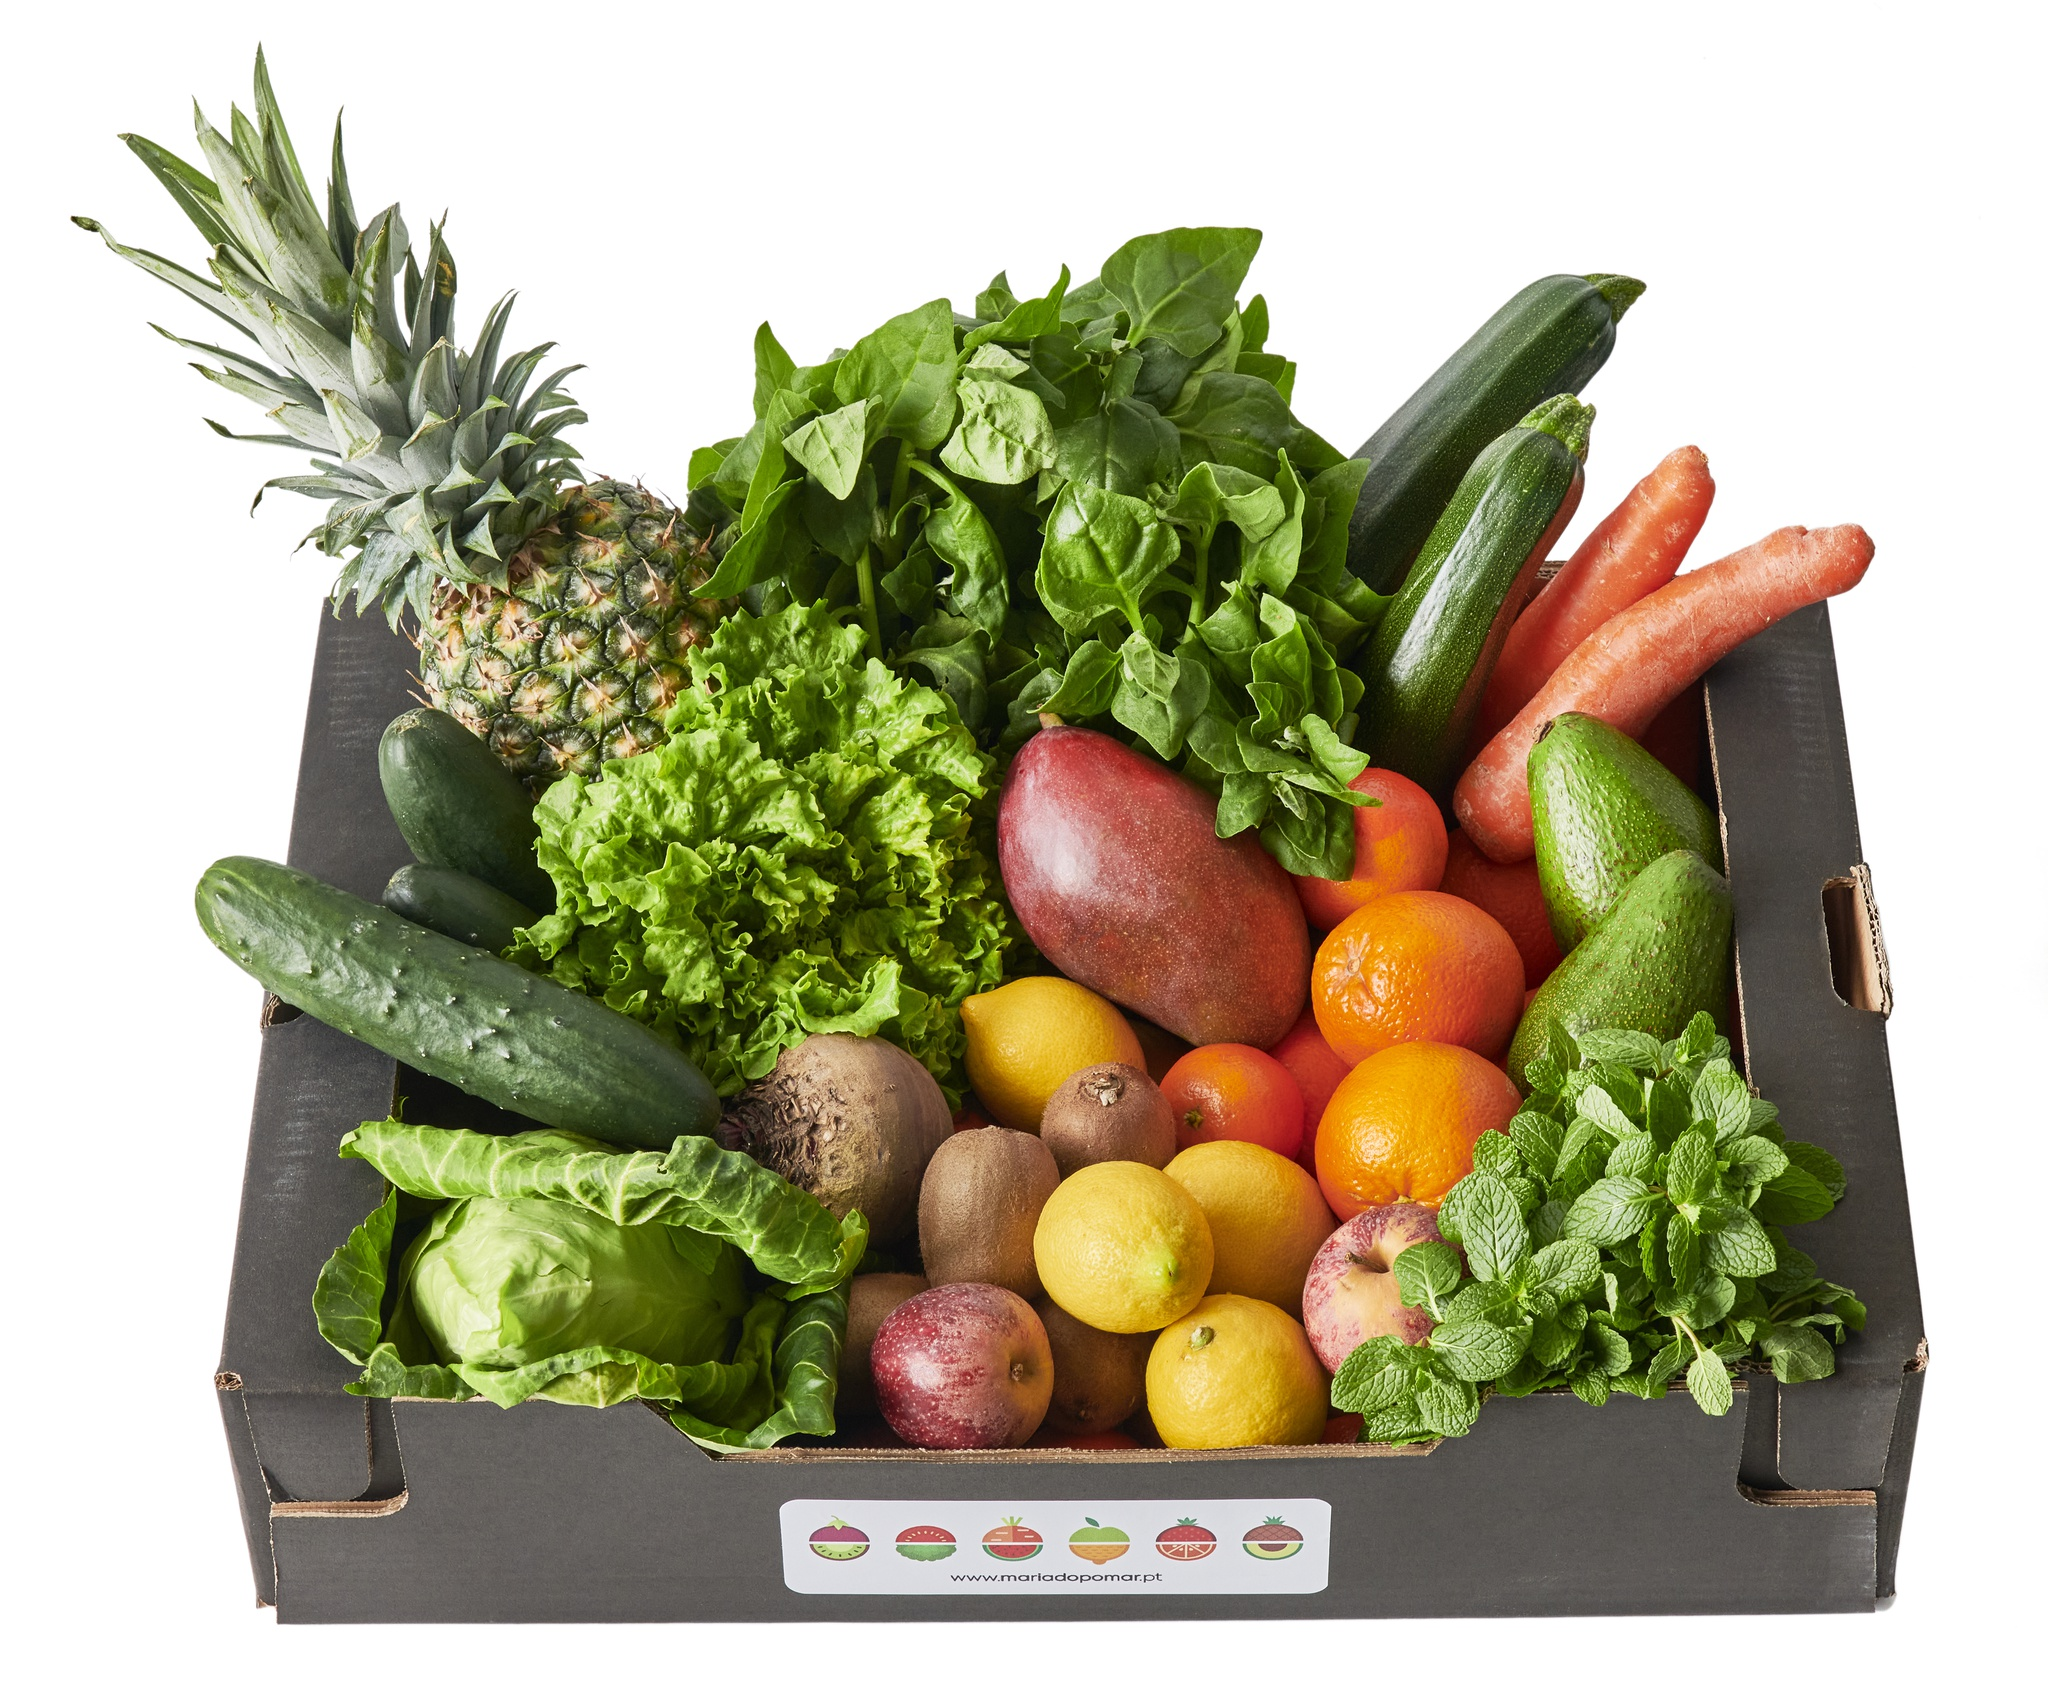
\includegraphics[scale=0.10]{Figures/0. General/cabaz.jpg}
  \caption{Cabaz de produtos sustentáveis}
  \label{Cabaz de produtos sustentáveis}
\end{figure}

\newpage

\subsection{Principais funcionalidades}
Optamos por organizar as funcionalidades da nossa aplicação em quatro categorias. Abaixo, apresentamos cada uma, com alguns exemplos específicos de funcionalidades:

\vspace{6pt}

\begin{itemize}

  \item \textbf{Users} \\
  Nesta categoria incluímos todas as funcionalidades relacionadas com utilizadores (não vendedores), tais como:
  \begin{itemize}
    \item \textbf{Registo de utilizador}\\ Um novo utilizador deve poder registar-se com os seus dados na nossa aplicação.
    \item \textbf{Alterar dados de perfil}\\ Um utilizador registado deve poder fazer a alteração dos seus dados de perfil.
    \item \textbf{Criar uma morada de entrega}\\ Um utilizador deve poder criar uma morada de entrega para a sua conta.
    \item \textbf{Apagar morada}\\ Um utilizador registado deve poder apagar as suas moradas de entrega.
    \item \textbf{Apagar registo}\\ Um utilizador registado deve poder apagar o seu registo.
  \end{itemize}

  \vspace{6pt}

  \item \textbf{Products} \\
  Nesta categoria incluímos todo o tipo de funcionalidades que envolvem os produtos:
  \begin{itemize}
      \item \textbf{Adicionar produto}\\ Um vendedor pode adicionar um produto novo para pôr á venda na sua loja.
      \item \textbf{Adicionar ao carrinho}\\ Um utilizador pode adicionar um produto que esteja á venda numa loja ao seu carrinho de compras.
      \item \textbf{Criar categoria}\\ Um vendedor pode adicionar uma nova categoria para os seus produtos.
      \item \textbf{Adicionar imagem}\\ Um vendedor pode adicionar uma imagem a uma galeria de imagens de um determinado produto.
      \item \textbf{Limpar o carrinho}\\ Um utilizador pode remover todos os produtos que adicionou ao seu carrinho de compras de uma só vez.
  \end{itemize}

  \newpage

  \item \textbf{Store} \\
  Nesta categoria incluímos todo o tipo de funcionalidades que envolvem as lojas:
  \begin{itemize}
    
    \item \textbf{Registo como vendedor}\\ Um utilizador normal deve poder registar-se como vendedor.
    \item \textbf{Criar nova loja}\\ Um vendedor pode criar uma nova loja.
    \item \textbf{Adicionar imagem}\\ Um vendedor pode adicionar uma imagem a uma galeria de imagens de uma determinada loja que lhe pertença.
    \item \textbf{Eliminar loja}\\ Um vendedor deve poder apagar uma loja que lhe pertença.
    \item \textbf{Modificar avaliaçao da loja}\\ Um utilizador deve poder modificar uma avaliação que fez no passado de uma loja que seja cliente.
\end{itemize}

\vspace{6pt}

\item \textbf{Orders} \\
Nesta categoria incluímos todo o tipo de funcionalidades que envolvem as encomendas:
\begin{itemize}
  \item \textbf{Fazer encomenda}\\ Um utilizador deve poder realizar uma encomenda dos produtos que tem no carrinho de compras.
  \item \textbf{Consultar estado da encomenda}\\ Um utilizador pode consultar o estado de uma encomenda que tenha feito.
  \item \textbf{Cancelar encomenda}\\ Um utilizador que tenha feito uma encomenda pode cancelá-la a qualquer momento desde que a encomenda não tenha ainda sido enviada.
  \item \textbf{Visualizar valor total}\\ Um utilizador deve poder visualizar o valor total de uma encomenda que tenha realizado.
  \item \textbf{Ordenar encomendas}\\ Um utilizador deve poder organizar todas as encomendas que realizou por data ou estado.
\end{itemize}
\end{itemize}
\newpage

% Capitulo 3
\section{Modelação da base de dados} \label{section: Modelacao}

\subsection{Diagramas, tabelas e modelos}
Com as funcionalidades da aplicação definidas o próximo passo foi modelar a base de dados criando as tabelas e desenhando o diagrama de Entidade-Relacionamento Estendido(EER) através da ferramenta \textit{MySQL Workbench}.

\subsubsection{Tabelas}

Criámos as tabelas tendo em conta as funcionalidades da aplicação:

\begin{itemize}

    \vspace{6pt}
    \item \textbf{user:}
     Dados dos utilizadores registados na aplicação.
    \begin{table}[H]
        \rowcolors{2}{gray!10}{white}
        \centering
        \begin{tabularx}{\linewidth}{XXXXX}
        \toprule
        \textbf{\color{color_scheme}Nome} & \textbf{\color{color_scheme}Tipo} & \textbf{\color{color_scheme}Atributos} & \textbf{\color{color_scheme}Padrão / Expressão}\\
        \midrule
        \texttt{user\_id} & \texttt{INT} & \texttt{PK - NN - AI} &\\
        \texttt{vendor\_id} & \texttt{INT}  & \texttt{FK}  & \texttt{NULL} \\
        \texttt{first\_name} & \texttt{VARCHAR(100)}  & \texttt{NN}  & \\
        \texttt{last\_name} & \texttt{VARCHAR(100)}  & \texttt{NN}  & \\
        \texttt{email} & \texttt{VARCHAR(100)}  & \texttt{NN - UQ}  & \\
        \texttt{deleted} & \texttt{TINYINT}  & \texttt{NN}  & \texttt{0} \\
        \bottomrule
        \end{tabularx}
        \label{table: user}
    \end{table}

    \vspace{3pt}
    \item \textbf{home\_address:}
    Moradas de entrega associadas aos utilizadores. 
    \begin{table}[H]
        \rowcolors{2}{gray!10}{white}
        \centering
        \begin{tabularx}{\linewidth}{XXXXX}
        \toprule
        \textbf{\color{color_scheme}Nome} & \textbf{\color{color_scheme}Tipo} & \textbf{\color{color_scheme}Atributos} & \textbf{\color{color_scheme}Padrão / Expressão}\\
        \midrule
        \texttt{home\_address\_id} & \texttt{INT} & \texttt{PK - NN - AI} &\\
        \texttt{user\_id} & \texttt{INT}  & \texttt{NN - FK}  &  \\
        \texttt{first\_name} & \texttt{VARCHAR(100)}  & \texttt{NN}  & \\
        \texttt{last\_name} & \texttt{VARCHAR(100)}  & \texttt{NN}  & \\
        \texttt{phone\_number} & \texttt{CHAR(9)}  & \texttt{NN - UQ}  & \\
        \texttt{street\_address} & \texttt{VARCHAR(100)}  & \texttt{NN}  & \\
        \texttt{postal\_code} & \texttt{CHAR(8)}  & \texttt{NN}  & \\
        \texttt{city} & \texttt{VARCHAR(100)}  & \texttt{NN}  & \\
        \texttt{comment} & \texttt{MEDIUMTEXT}  &  & \\
        \texttt{deleted} & \texttt{TINYINT}  & \texttt{NN}  & \texttt{0} \\
        \bottomrule
        \end{tabularx}
        \label{table: address_home}
    \end{table}

    \newpage

    \item \textbf{product:}
    Produtos inseridos pelos vendedores. 
    \begin{table}[H]
        \rowcolors{2}{gray!10}{white}
        \centering
        \begin{tabularx}{\linewidth}{XXXXX}
        \toprule
        \textbf{\color{color_scheme}Nome} & \textbf{\color{color_scheme}Tipo} & \textbf{\color{color_scheme}Atributos} & \textbf{\color{color_scheme}Padrão / Expressão}\\
        \midrule
        \texttt{product\_id} & \texttt{INT} & \texttt{PK - NN - AI} &\\
        \texttt{product\_name} & \texttt{VARCHAR(100)}  & \texttt{NN}  & \\
        \texttt{description} & \texttt{MEDIUMTEXT}  & \texttt{NN}  & \\
        \texttt{discount} & \texttt{DOUBLE}  & \texttt{NN - UQ}  & \texttt{0.0}\\
        \texttt{image\_link} & \texttt{VARCHAR(250)}  &  & \\
        \texttt{price} & \texttt{DOUBLE}  & \texttt{NN - UQ}  & \\
        \texttt{stock} & \texttt{INT}  & \texttt{NN - UQ}  & \\
        \texttt{is\_unit} & \texttt{TINYINT}  & \texttt{NN - UQ} & \texttt{0} \\
        \bottomrule
        \end{tabularx}
        \label{table: product}
    \end{table}

    \vspace{3pt}

    \item \textbf{category:}
    Categorias dos produtos. 
    \begin{table}[H]
        \rowcolors{2}{gray!10}{white}
        \centering
        \begin{tabularx}{\linewidth}{XXXXX}
        \toprule
        \textbf{\color{color_scheme}Nome} & \textbf{\color{color_scheme}Tipo} & \textbf{\color{color_scheme}Atributos} & \textbf{\color{color_scheme}Padrão / Expressão}\\
        \midrule
        \texttt{category\_id} & \texttt{INT} & \texttt{PK - NN - AI} &\\
        \texttt{category\_name} & \texttt{VARCHAR(100)}  & \texttt{NN}  & \\
        \bottomrule
        \end{tabularx}
        \label{table: categories}
    \end{table}

    \vspace{3pt}

    \item \textbf{product\_gallery:}
    Galeria de imagens dos produtos. 
    \begin{table}[H]
        \rowcolors{2}{gray!10}{white}
        \centering
        \begin{tabularx}{\linewidth}{XXXXX}
        \toprule
        \textbf{\color{color_scheme}Nome} & \textbf{\color{color_scheme}Tipo} & \textbf{\color{color_scheme}Atributos} & \textbf{\color{color_scheme}Padrão / Expressão}\\
        \midrule
        \texttt{product\_gallery\_id} & \texttt{INT} & \texttt{PK - NN - AI} &\\
        \texttt{product\_id} & \texttt{INT} & \texttt{NN - FK} & \\
        \texttt{image\_link} & \texttt{VARCHAR(250)}  & \texttt{NN} & \\
        \bottomrule
        \end{tabularx}
        \label{table: product_gallery}
    \end{table}

    \vspace{3pt}

    \item \textbf{product\_category:}
    Ligação entre produtos e categorias. 
    \begin{table}[H]
        \rowcolors{2}{gray!10}{white}
        \centering
        \begin{tabularx}{\linewidth}{XXXXX}
        \toprule
        \textbf{\color{color_scheme}Nome} & \textbf{\color{color_scheme}Tipo} & \textbf{\color{color_scheme}Atributos} & \textbf{\color{color_scheme}Padrão / Expressão}\\
        \midrule
        \texttt{product\_id} & \texttt{INT} & \texttt{PK - NN - FK} &\\
        \texttt{category\_id} & \texttt{INT} & \texttt{PK - NN - FK} &\\
        \bottomrule
        \end{tabularx}
        \label{table: product_categories}
    \end{table}
   
    \newpage

    \item \textbf{product\_review:}
    Avaliações dos produtos. 
    \begin{table}[H]
        \rowcolors{2}{gray!10}{white}
        \centering
        \begin{tabularx}{\linewidth}{XXXXX}
        \toprule
        \textbf{\color{color_scheme}Nome} & \textbf{\color{color_scheme}Tipo} & \textbf{\color{color_scheme}Atributos} & \textbf{\color{color_scheme}Padrão / Expressão}\\
        \midrule
        \texttt{product\_review\_id} & \texttt{INT} & \texttt{PK - NN - AI} &\\
        \texttt{user\_id} & \texttt{INT} & \texttt{NN - FK} &\\
        \texttt{product\_id} & \texttt{INT} & \texttt{NN - FK} &\\
        \texttt{rating} & \texttt{INT}  & \texttt{NN}  & \\
        \texttt{created} & \texttt{TIMESTAMP}  &  & \texttt{CURRENT\_TIMESTAMP}\\
        \texttt{comment} & \texttt{MEDIUMTEXT}  & \texttt{NN} & \\
        \bottomrule
        \end{tabularx}
        \label{table: product_reviews}
    \end{table}

    \item \textbf{store:}
    Lojas registadas pelos vendedores. 
    \begin{table}[H]
        \rowcolors{2}{gray!10}{white}
        \centering
        \begin{tabularx}{\linewidth}{XXXXX}
        \toprule
        \textbf{\color{color_scheme}Nome} & \textbf{\color{color_scheme}Tipo} & \textbf{\color{color_scheme}Atributos} & \textbf{\color{color_scheme}Padrão / Expressão}\\
        \midrule
        \texttt{store\_id} & \texttt{INT} & \texttt{PK - NN - AI} &\\
        \texttt{vendor\_id} & \texttt{INT} & \texttt{NN - FK} & \\
        \texttt{store\_name} & \texttt{VARCHAR(100)}  & \texttt{NN - UQ} & \\
        \texttt{store\_phone} & \texttt{VARCHAR(9)}  & \texttt{NN} & \\
        \texttt{store\_email} & \texttt{VARCHAR(100)}  & \texttt{NN - UQ} & \\
        \texttt{description} & \texttt{MEDIUMTEXT}  & \texttt{NN} & \\
        \texttt{profile\_picture} & \texttt{VARCHAR(250)} &  & \\
        \texttt{street\_address} & \texttt{VARCHAR(100)} & \texttt{NN} & \\
        \texttt{city} & \texttt{VARCHAR(100)} & \texttt{NN} & \\
        \texttt{postal\_code} & \texttt{CHAR(8)} & \texttt{NN} & \\
        \texttt{deleted} & \texttt{TINYINT}  & \texttt{NN}  & \texttt{0} \\
        \bottomrule
        \end{tabularx}
        \label{table: store}
    \end{table}

    \item \textbf{store\_review:}
    Avaliações das lojas. 
    \begin{table}[H]
        \rowcolors{2}{gray!10}{white}
        \centering
        \begin{tabularx}{\linewidth}{XXXXX}
        \toprule
        \textbf{\color{color_scheme}Nome} & \textbf{\color{color_scheme}Tipo} & \textbf{\color{color_scheme}Atributos} & \textbf{\color{color_scheme}Padrão / Expressão}\\
        \midrule
        \texttt{store\_review\_id} & \texttt{INT} & \texttt{PK - NN - AI} &\\
        \texttt{user\_id} & \texttt{INT} & \texttt{NN - FK} &\\
        \texttt{store\_id} & \texttt{INT} & \texttt{NN - FK} &\\
        \texttt{rating} & \texttt{INT}  & \texttt{NN}  & \\
        \texttt{created} & \texttt{TIMESTAMP}  &  & \texttt{CURRENT\_TIMESTAMP}\\
        \texttt{comment} & \texttt{MEDIUMTEXT}  & \texttt{NN} & \\
        \bottomrule
        \end{tabularx}
        \label{table: store_reviews}
    \end{table}

    \newpage

    \item \textbf{store\_gallery:}
    Galeria de imagens das lojas. 
    \begin{table}[H]
        \rowcolors{2}{gray!10}{white}
        \centering
        \begin{tabularx}{\linewidth}{XXXXX}
        \toprule
        \textbf{\color{color_scheme}Nome} & \textbf{\color{color_scheme}Tipo} & \textbf{\color{color_scheme}Atributos} & \textbf{\color{color_scheme}Padrão / Expressão}\\
        \midrule
        \texttt{store\_gallery\_id} & \texttt{INT} & \texttt{PK - NN - AI} &\\
        \texttt{store\_id} & \texttt{INT} & \texttt{NN - FK} & \\
        \texttt{image\_link} & \texttt{VARCHAR(250)}  & \texttt{NN} & \\
        \bottomrule
        \end{tabularx}
        \label{table: store_gallery}
    \end{table}

    \item \textbf{vendor:}
    Utilizadores que estão registados como vendedores.
    \begin{table}[H]
        \rowcolors{2}{gray!10}{white}
        \centering
        \begin{tabularx}{\linewidth}{XXXXX}
        \toprule
        \textbf{\color{color_scheme}Nome} & \textbf{\color{color_scheme}Tipo} & \textbf{\color{color_scheme}Atributos} & \textbf{\color{color_scheme}Padrão / Expressão}\\
        \midrule
        \texttt{vendor\_id} & \texttt{INT} & \texttt{PK - NN - AI} &\\
        \texttt{user\_id} & \texttt{INT} & \texttt{NN - FK} & \\
        \texttt{nif} & \texttt{CHAR(9)} & \texttt{NN - UQ} & \\
        \texttt{deleted} & \texttt{TINYINT}  & \texttt{NN}  & \texttt{0} \\
        \bottomrule
        \end{tabularx}
        \label{table: vendor}
    \end{table}

    \item \textbf{order:}
    Encomendas feitas pelos utilizadores. 
    \begin{table}[H]
        \rowcolors{2}{gray!10}{white}
        \centering
        \begin{tabularx}{\linewidth}{XXXXX}
        \toprule
        \textbf{\color{color_scheme}Nome} & \textbf{\color{color_scheme}Tipo} & \textbf{\color{color_scheme}Atributos} & \textbf{\color{color_scheme}Padrão / Expressão}\\
        \midrule
        \texttt{order\_id} & \texttt{INT} & \texttt{PK - NN - AI} &\\
        \texttt{user\_id} & \texttt{INT}  & \texttt{NN - FK}  &  \\
        \texttt{street\_address} & \texttt{VARCHAR(100)}  & \texttt{NN}  & \\
        \texttt{postal\_code} & \texttt{CHAR(8)}  & \texttt{NN}  & \\
        \texttt{city} & \texttt{VARCHAR(100)}  & \texttt{NN}  & \\
        \texttt{created} & \texttt{TIMESTAMP}  &  & \texttt{CURRENT\_TIMESTAMP}\\
        \texttt{comment} & \texttt{MEDIUMTEXT}  &  & \\
        \texttt{status} & \texttt{ENUM()}  & \texttt{NN}  &  \\
        \bottomrule
        \end{tabularx}
        \label{table: order}
    \end{table}

        \item \textbf{order\_product:}
        Produtos que fazem parte das encomendas. 
        \begin{table}[H]
            \rowcolors{2}{gray!10}{white}
            \centering
            \begin{tabularx}{\linewidth}{XXXXX}
            \toprule
            \textbf{\color{color_scheme}Nome} & \textbf{\color{color_scheme}Tipo} & \textbf{\color{color_scheme}Atributos} & \textbf{\color{color_scheme}Padrão / Expressão}\\
            \midrule
            \texttt{order\_product\_id} & \texttt{INT} & \texttt{PK - NN - AI} &\\
            \texttt{order\_id} & \texttt{INT}  & \texttt{NN - FK}  &  \\
            \texttt{product\_id} & \texttt{INT}  & \texttt{NN - FK}  &  \\
            \texttt{price} & \texttt{DOUBLE}  & \texttt{NN}  & \\
            \texttt{discount} & \texttt{DOUBLE}  & \texttt{NN}  & \texttt{0.0}\\
            \bottomrule
            \end{tabularx}
            \label{table: order_product}
        \end{table}

\end{itemize}

\newpage

\subsubsection{Diagrama EER}
Introduzimos as tabelas criadas no \textit{MySQL Workbench} e criámos os relacionamentos entre elas utilizando as chaves estrangeiras:

\vspace{12pt}

\begin{figure}[H]
    \centering
    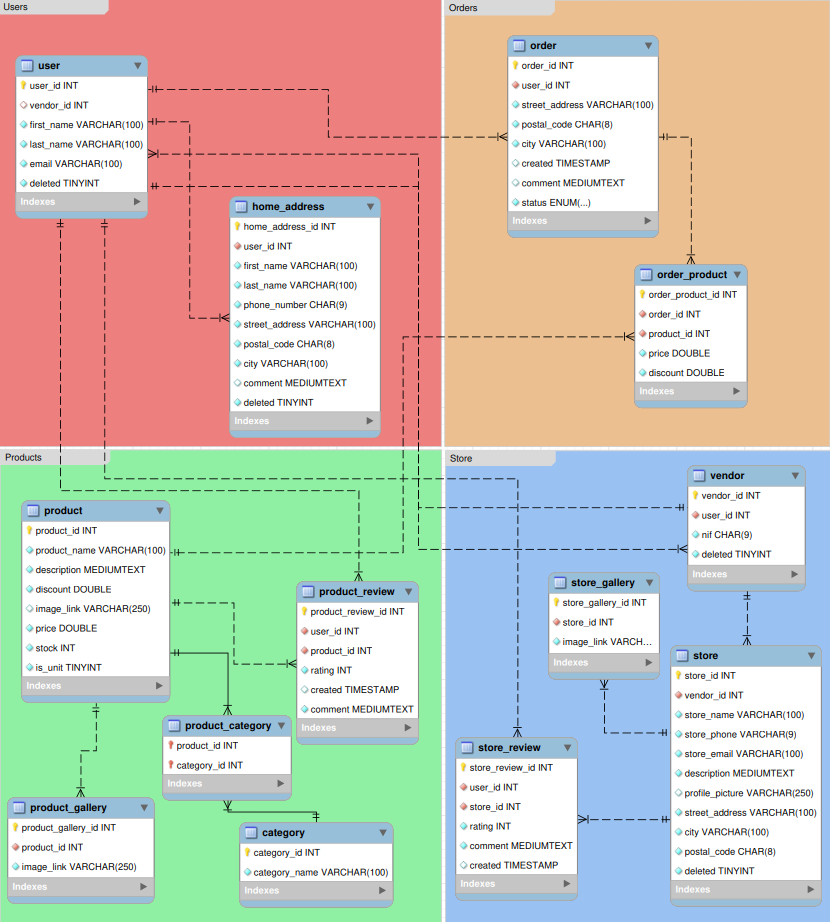
\includegraphics[width=\textwidth]{Figures/0. General/diagram.png}
    \caption{Diagrama EER}
    \label{Diagrama EER}
\end{figure}

\newpage



\newpage

% Capitulo 4
\section{Consultas á base de dados} \label{section: Consultas}
teste
\newpage

% Capitulo 5
\section{Conclusão} \label{section: Conclusao}
Realizar este trabalho permitiu o início do projeto final de curso, forçando o grupo a uma reflexão e debate de ideias.
\par \vspace{6pt}
Definidos os objetivos do projeto final e estabelecidas as principais funcionalidades da aplicação, iniciou-se a modelação da base de dados a utilizar. Esta modelação levou o grupo a debater sobre as funcionalidades escolhidas, a sua dificuldade e a consonância dos objetivos definidos com a ambição do projeto.
\par \vspace{6pt}
Com o desenvolvimento deste modelo da base de dados do projeto final, foi possível ao grupo aprender, praticar e compreender o que está por detrás de uma plataforma para lojas online.
\newpage

% contains inspiration for formatting tables, images, text citations etc.
\section{This is a section} \pagenumbering{roman}
\subsection{This is a subsection}

\subsubsection{This is a subsubsection}
This section contains some templates that can be used to create a uniform style within the document. It also shows of the overall formatting of the template, created using the predefined styles from the \texttt{settings.tex} file.

\subsection{General formatting}
Bullet lists are also changed globally, for a maximum of 3 levels:

\begin{itemize}
    \item Item 1
    \item Item 2
    \begin{itemize}
        \item subitem 1
        \begin{itemize}
            \item subsubitem 1
            \item subsubitem 2
        \end{itemize}
    \end{itemize}
    \item Item 3
\end{itemize}

Similarly numbered lists are also changed document wide:

\begin{enumerate}
    \item Item 1
    \item Item 2
    \begin{enumerate}
        \item subitem 1
        \begin{enumerate}
            \item subsubitem 1
            \item subsubitem 2
        \end{enumerate}
    \end{enumerate}
    \item Item 3
\end{enumerate}

\newpage

\subsection{Tables and figures}
The following table, \cref{table: style 1}, shows a possible format for tables in this document. Alternatively, one can also use the black and white version of this, shown in \cref{table: style 2}. Note that caption labels are in the format \textbf{\textcolor{color_scheme}{Table x.y:} }
\begin{table}[ht]
\rowcolors{2}{color_scheme!10}{white}
\centering
\caption{A table without vertical lines.}
\begin{tabular}[t]{ccccc}
\toprule
\color{color_scheme}\textbf{Column 1}&\color{color_scheme}\textbf{Column 2}&\color{color_scheme}\textbf{Column 3}&\color{color_scheme}\textbf{Column 4}&\color{color_scheme}\textbf{Column 5}\\
\midrule
Entry 1&1&2&3&4\\
Entry 2&1&2&3&4\\
Entry 3&1&2&3&4\\
Entry 4&1&2&3&4\\
\bottomrule
\end{tabular}
\label{table: style 1}
\end{table}

\begin{table}[ht]
\rowcolors{2}{gray!10}{white}
\centering
\caption{A table without vertical lines.}
\begin{tabular}[t]{ccccc}
\toprule
\textbf{Column 1}&\textbf{Column 2}&\textbf{Column 3}&\textbf{Column 4}&\textbf{Column 5}\\
\midrule
Entry 1&1&2&3&4\\
Entry 2&1&2&3&4\\
Entry 3&1&2&3&4\\
Entry 4&1&2&3&4\\
\bottomrule
\end{tabular}
\label{table: style 2}
\end{table}

% For normal, single image figures, the standard \texttt{\textbackslash begin\{figure\}} environment can be used. For multi-image figures, one could use either the \texttt{\textbackslash begin\{subfigure\}} environment to get a main caption with 3 subcaptions like \cref{fig: three images} or the \texttt{\textbackslash begin\{minipage\}} environment to get 3 independent captions like \cref{fig: style 2 image a} - \ref{fig: style 2 image c}

\begin{figure}[H]
     \centering
     \begin{subfigure}[b]{0.3\textwidth}
         \centering
         \includegraphics[width=\textwidth]{example-image-a}
         \caption{image a}
         \label{fig: style 1 image a}
     \end{subfigure}
     \hfill
     \begin{subfigure}[b]{0.3\textwidth}
         \centering
         \includegraphics[width=\textwidth]{example-image-b}
         \caption{image b}
         \label{fig: style 1 image b}
     \end{subfigure}
     \hfill
     \begin{subfigure}[b]{0.3\textwidth}
         \centering
         \includegraphics[width=\textwidth]{example-image-c}
         \caption{image c}
         \label{fig: style 1 image c}
     \end{subfigure}
        \caption{Three images}
        \label{fig: three images}
\end{figure}

\begin{figure}[H]
\centering
\begin{minipage}{0.3\textwidth}
  \centering
  \includegraphics[width=\textwidth]{example-image-a}
  \captionof{figure}{image a}
  \label{fig: style 2 image a}
\end{minipage}
\hfill
\begin{minipage}{0.3\textwidth}
  \centering
  \includegraphics[width=\textwidth]{example-image-b}
  \captionof{figure}{image b}
  \label{fig: style 2 image b}
\end{minipage}
\hfill
\begin{minipage}{0.3\textwidth}
  \centering
  \includegraphics[width=\textwidth]{example-image-c}
  \captionof{figure}{image c}
  \label{fig: style 2 image c}
\end{minipage}
\end{figure} % Feel free to remove / comment out
\newpage

% Generates a list of symbols table
\section*{list of symbols} \label{section: symbols}

\begin{table}[ht]
\rowcolors{2}{gray!10}{white}
\centering
\caption{list of symbols}
\begin{tabular}[t]
{m{0.1\textwidth}m{0.25\textwidth}m{0.25\textwidth}m{0.2\textwidth}}
\toprule
\textbf{Symbol}&\textbf{dimension}&\textbf{Unit}&\textbf{Unit abbreviation}\\
\midrule
1&2&3&4\\
1&2&3&4\\
1&2&3&4\\
1&2&3&4\\
\bottomrule
\end{tabular}
\end{table}
\newpage


% Creates references using the Biblatex 
% \bibliographystyle{unsrt}
% \bibliography{General/References.bib}
% \newpage

% \appendix % Any section after this command will have a letter as an index

% Adds an appendix entry
% \section{Apêndice A - Referências} \label{section: appendix A title}
% \lipsum[1-8]
texto
% \newpage

\end{document}
